\section{Results}
\label{sec:results}

\subsection{RQ1: clustering beyond births}
\paragraph{A north--south gradient} Over 1975--2005, England produced \engRate{} players for every 10\,000 boys born. London (\londonRate{}) and the North West (\nwRate{}) produced the most and the South West (\swRate{}) and the South East (\seRate{}) the least, a ratio of \regionRatio{} between the highest and the lowest region (Table~\ref{tab:regions}, Figure~\ref{fig:regions}). \nRegionsSig{} of the 9 regions differ from the England rate at $p<0.05$; Yorkshire and the Humber and the West Midlands do not.

\begin{table}[ht]
\centering
\caption{Players per region against expectations from male births, 1975--2005. SR with exact Poisson 95\% confidence interval and test of SR $=1$.}
\label{tab:regions}
\tbl{regions.tex}
\end{table}

\begin{figure}[ht]
\centering
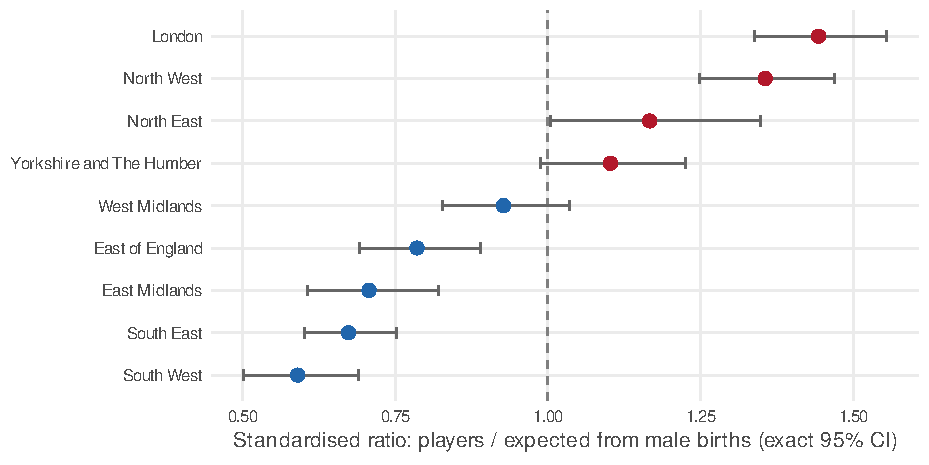
\includegraphics[width=0.85\textwidth]{figures/fig_regions.pdf}
\caption{Standardised ratio by region with exact 95\% confidence intervals. Red: more players than births predict.}
\label{fig:regions}
\end{figure}

\paragraph{Clustering within regions} The point-pattern test asks whether, beyond these differences in where boys are born, players' birthplaces lie closer together than births would place them. They do, modestly (Table~\ref{tab:ltests}, Figure~\ref{fig:lfunction}). The observed $L(r)-r$ lies about \lExcess{}\,km above zero at most distances up to 60\,km. The DCLF test is significant over 0--60\,km ($p=\lDCLFall$) and over 20--60\,km ($p=\lDCLFfar$); the MAD test, which looks at the single largest deviation, gives $p=\lMADall$ and $p=\lMADfar$. A pattern drawn from births alone gives $p=\lNullAll$ and $p=\lNullFar$, so the method does not create clustering by itself. The curve leaves the global envelope only at 1--3\,km, the distances most affected by shared town coordinates and maternity hospitals, and we do not interpret that.

\textbf{H0 is rejected}: players are not born in proportion to births. The evidence is strong at the scale of regions and modest within them.

\begin{table}[ht]
\centering
\caption{Global envelope tests of the inhomogeneous $L$-function against the births intensity.}
\label{tab:ltests}
\tbl{ltests.tex}
\end{table}

\begin{figure}[ht]
\centering
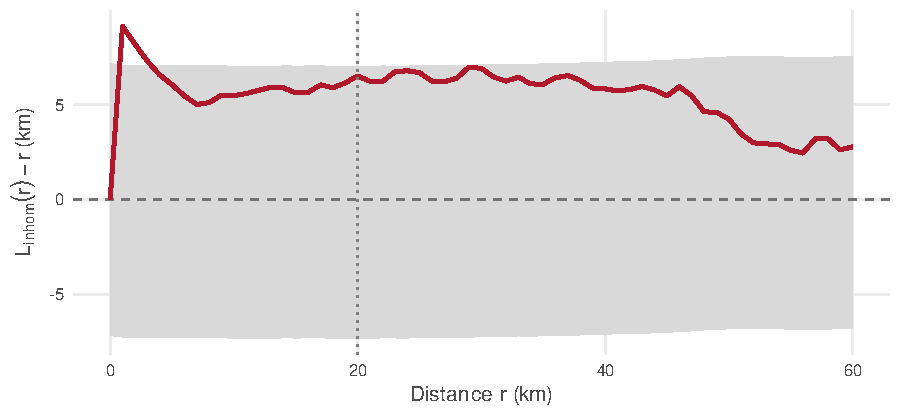
\includegraphics[width=0.8\textwidth]{figures/fig_lfunction.pdf}
\caption{Inhomogeneous $L$-function of the \nTown{} town-level birthplaces, $L(r)-r$ (red), with the 95\% global envelope of \nSim{} patterns drawn from the births intensity (grey). Values above zero mean more clustering than births predict. The dotted line marks 20\,km, below which shared town coordinates and maternity hospitals affect the curve.}
\label{fig:lfunction}
\end{figure}

\FloatBarrier
\subsection{RQ2: hotspots and coldspots}
\paragraph{Global clustering} Across the \nTTWA{} TTWAs, areas that produce many players lie next to other high areas and low areas next to low ones: EB Moran's $I = \moranTTWA$ ($p=\moranTTWAp$) with shared-border neighbours and \moranTTWAknn{} with 6 nearest neighbours (Table~\ref{tab:moran}). The clustering is much weaker across local authorities ($I$ from \moranLADlo{} to \moranLADhi) and 20\,km hexagons, the smaller areas in which the hospital effect and small numbers add noise.

\begin{table}[ht]
\centering
\caption{Global EB Moran's $I$ (\nSim{} permutations) and the number of local $G_i^*$ hot and cold clusters (\nPerm{} permutations) by set of areas and neighbour definition.}
\label{tab:moran}
\tbl{moran.tex}
\end{table}

\paragraph{Where} After smoothing, the SR ranges from \ebMin{} to \ebMax{} (Figure~\ref{fig:maps}a, Table~\ref{tab:toparea} in the appendix). Liverpool is the most productive area, with \liverpoolO{} players against \liverpoolE{} expected (SR$_{EB}$ \liverpoolSR). High values form a belt from Merseyside and Cheshire through Lancashire and Greater Manchester to South Yorkshire, with London and the North East also above expectation. Low values run along the south coast, through Kent, Sussex, Hampshire and Dorset, and across the rural South West and East Anglia.

\paragraph{Local clusters} At unadjusted $p<0.05$, $G_i^*$ finds \nHot{} hot and \nCold{} cold TTWA clusters (Table~\ref{tab:gi}, Figure~\ref{fig:maps}b). The hot clusters lie in Lancashire, Greater Manchester and Yorkshire, the cold clusters in Kent, Sussex, Hampshire and Wiltshire. The strongest is \giTopName{} ($z=\giTopZ$), whose own SR is close to expectation but which is surrounded by the high areas of Liverpool, Manchester and Preston; LISA classes it as low-high. After FDR control no single TTWA reaches $q<0.05$; the strongest, \giTopName{}, has $q=\giTopQ$. Under the normal approximation, five TTWAs pass $q<0.05$: \hotNormList.

\textbf{H1 is supported for the overall pattern but only weakly for named areas.} Players come from a gradient across the country, highest in the North West, rather than from a few isolated hotspots.

\begin{figure}[ht]
\centering
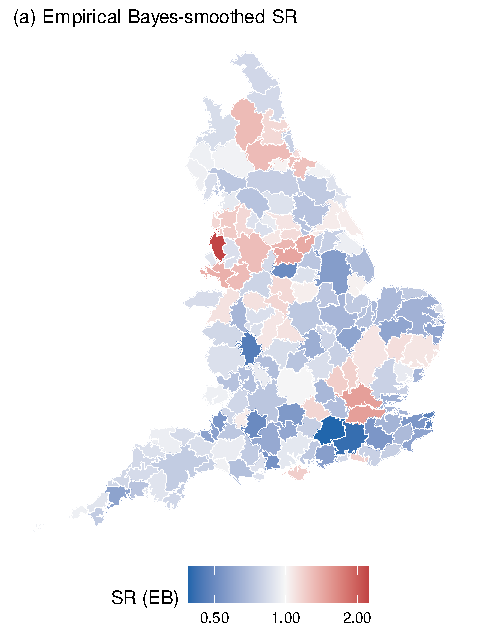
\includegraphics[width=0.48\textwidth]{figures/fig_ttwa_sr.pdf}\hfill
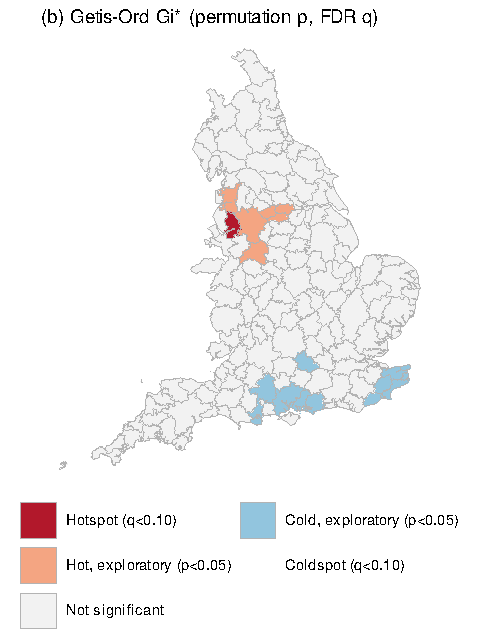
\includegraphics[width=0.48\textwidth]{figures/fig_ttwa_gi.pdf}
\caption{Travel to Work Areas. (a) Empirical Bayes-smoothed standardised ratio. (b) Getis-Ord $G_i^*$ clusters with shared-border neighbours and \nPerm{} permutations; $q$ is the Benjamini-Hochberg adjusted $p$-value.}
\label{fig:maps}
\end{figure}

\begin{table}[ht]
\centering
\caption{TTWAs with a $G_i^*$ hot or cold cluster at unadjusted $p<0.05$ (shared-border neighbours, \nPerm{} permutations). $q$: Benjamini-Hochberg adjusted.}
\label{tab:gi}
\tbl{gi.tex}
\end{table}

\FloatBarrier
\subsection{RQ3: what explains the differences}
\paragraph{Model checks} The data are overdispersed (Pearson dispersion \dispersion{} in a Poisson model), so we use the negative binomial. Variance inflation factors are at most \vifMax{}, although urban share and distance to a club are correlated ($r=\corUrbanDist$). Region effects improve the fit (likelihood ratio $\chi^2=\lrChi$, \lrDf{} df, $p=\lrP$; AIC \aicOne{} for M1 and \aicTwo{} for M2). The residuals of M1 are spatially autocorrelated (Moran's $I=\resMoranOne$, $p=\resMoranOneP$); those of M2 are not ($I=\resMoranTwo$, $p=\resMoranTwoP$). The Lagrange multiplier tests give no reason for a spatial model (all $p \ge \lmPmin$), and the fitted spatial error and lag parameters are close to zero ($\lambda=\semLambda$, $p=\semP$; $\rho=\slmRho$, $p=\slmP$). Region effects absorb the spatial structure.

\paragraph{Effects} In M2, each extra 10\,km between an area and its nearest professional club lowers the rate of players by \distPct\% (rate ratio \distRR, 95\% CI \distLo--\distHi, $p\,\distP$; Table~\ref{tab:models}, Figure~\ref{fig:models}). In the spatial error and lag models the distance coefficient is also significant ($p=\spatialDistP$). Deprivation appears to raise production in M1 (rate ratio \imdRRmOne{} per 10 IMD points, $p=\imdPmOne$), but the effect disappears once region is included (\imdRR, $p=\imdP$): deprived areas are mostly in the North, which produces more players for reasons that the region effects capture. Urban share has no effect (\urbRR, $p=\urbP$). The region effects, relative to the West Midlands, keep a north--south order after the covariates: \nwRR{} for the North West and \neRR{} for the North East against \seRR{} for the South East and \swRR{} for the South West (Table~\ref{tab:regionfx} in the appendix).

\begin{table}[ht]
\centering
\caption{Negative binomial models of players per TTWA with offset $\log E$. Rate ratios per 10\,km, 10 IMD points and 10 percentage points of urban share.}
\label{tab:models}
\tbl{models.tex}
\end{table}

\begin{figure}[ht]
\centering
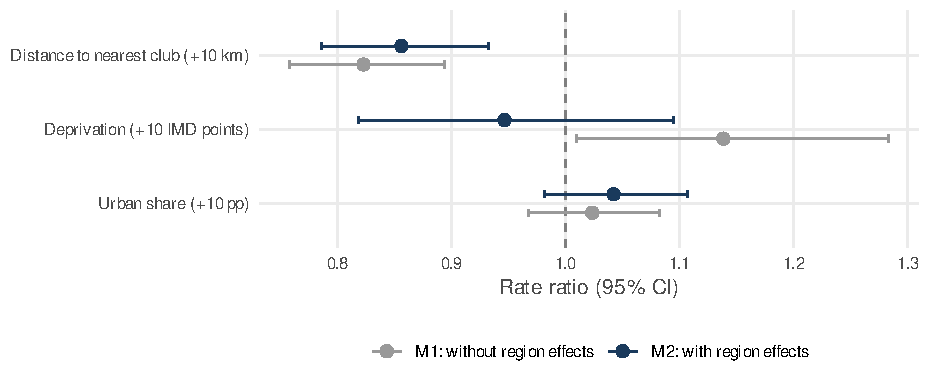
\includegraphics[width=0.85\textwidth]{figures/fig_models.pdf}
\caption{Rate ratios with 95\% confidence intervals, without (M1) and with (M2) region effects. The deprivation effect in M1 is explained by region.}
\label{fig:models}
\end{figure}

\paragraph{Elite academies} For the \nAcadPlayers{} players born 1996--2005, distance to any professional club has a stronger effect than for the full sample (rate ratio \clubYoungRR, 95\% CI \clubYoungLo--\clubYoungHi, $p\,\clubYoungP$), whereas distance to the nearest Category 1 academy has none (\acadRR, $p=\acadP$; Table~\ref{tab:academy}). With both in the model, club distance keeps its effect (\bothClubRR) and academy distance stays null (\bothAcadRR, $p=\bothAcadP$). The two distances are correlated ($r=\acadCor$) but differ in size: the median area is \clubDistMedYoung{}\,km from a club and \acadDistMed{}\,km from a Category 1 academy.

\begin{table}[ht]
\centering
\caption{Academy-era sub-model, players born 1996--2005. Negative binomial with deprivation, urban share and region effects; rate ratios per 10\,km.}
\label{tab:academy}
\tbl{academy.tex}
\end{table}

\textbf{H2 is supported for proximity to professional clubs only}, not for deprivation once region is included, not for urbanisation and not for elite academies.

\FloatBarrier
\subsection{Robustness}
The distance effect is significant at $p<0.05$ in \nRobustSig{} of the \nRobust{} model variants (Table~\ref{tab:robust}, Figure~\ref{fig:robust}). It holds with certain evidence only (\distRRCertain), for Premier League players only (\distRRPremier), with a total-population baseline (\distRRPop) and without the five largest cities (\distRRNoCities). It is weaker for players born 1975--89 (\distRROld, $p=\distPOld$) and stronger for those born 1990--2005 (\distRRYoung, $p\,\distPYoung$). It is not significant across local authorities (\distRRLAD, $p=\distPLAD$), where deprivation and urban share instead become significant; the hospital effect makes local authorities the least reliable set of areas (Section~\ref{sec:units}).

\begin{table}[ht]
\centering
\caption{Robustness of the main model (M2). Rate ratio ($p$) per 10\,km, 10 IMD points and 10 percentage points of urban share.}
\label{tab:robust}
\tbl{robust.tex}
\end{table}

\begin{figure}[ht]
\centering
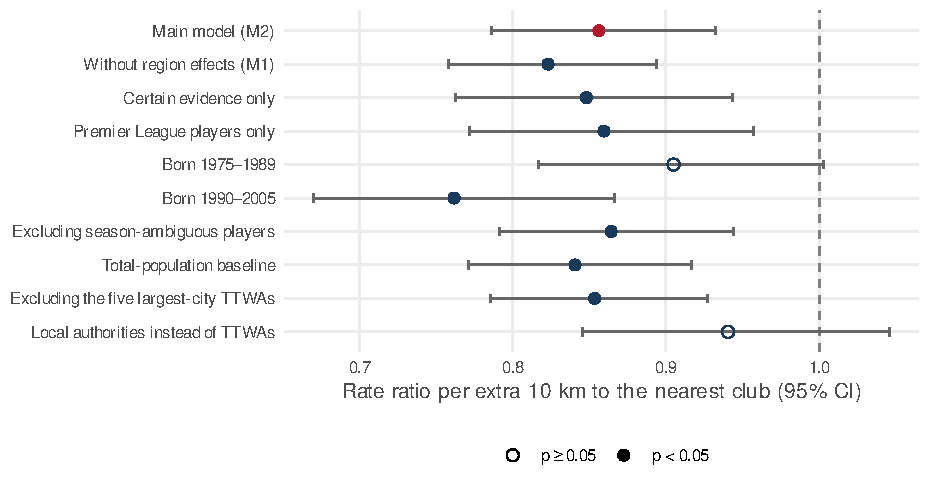
\includegraphics[width=0.85\textwidth]{figures/fig_robustness.pdf}
\caption{Rate ratio per extra 10\,km to the nearest professional club across model variants, with 95\% confidence intervals. Red: main model.}
\label{fig:robust}
\end{figure}

\FloatBarrier
\subsection{RQ4: players born outside England}
\nOutsideEngland{} of the \nStudy{} study players (\shareOutsideEngland\%) were born outside England, in \nCountries{} countries and UK nations: \nOtherUK{} (\shareOtherUK\%) in Scotland, Wales and Northern Ireland and \nOutsideUK{} (\shareOutsideUK\%) outside the UK (Table~\ref{tab:countries}). France, Scotland, Ireland and Spain supply the most. Relative to population, the small football nations lead: \topHeadName{} with \topHeadRate{} players per million people, and Ireland, Scotland and Wales with more than 40 (Figure~\ref{fig:world}).

The supply changed between cohorts. Scottish-born players fell from \scotOld{} in the 1975--89 cohort to \scotNew{} in the 1990--2005 cohort, more than any other country, while Germany and Belgium rose. Among players born outside the UK, Europe's share rose from \eurOld\% to \eurNew\%, and Africa's fell from \afrOld\% to \afrNew\%. England's share of all study players rose from \engShareOld\% to \engShareNew\%.

\begin{table}[ht]
\centering
\caption{The 15 countries and UK nations outside England with the most study players. Per million: mean national population 1975--2005 (no separate series for Northern Ireland).}
\label{tab:countries}
\tbl{countries.tex}
\end{table}

\begin{figure}[ht]
\centering
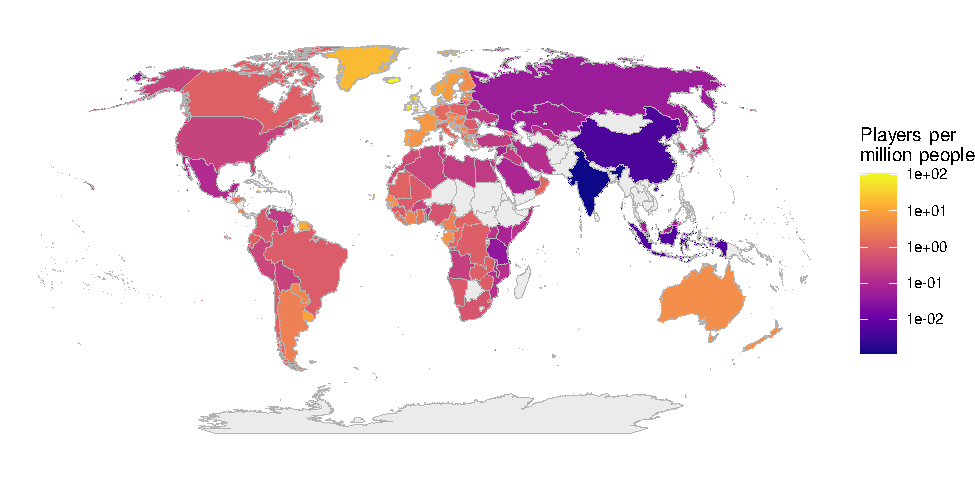
\includegraphics[width=\textwidth]{figures/fig_world.pdf}
\caption{Study players born outside England per million national population (mean 1975--2005), log scale. Grey: no study player or no population data.}
\label{fig:world}
\end{figure}
\FloatBarrier
